\section{Постановка задач}
Предварительно оптимизировать молекулярную структуру с помощью программы Avogadro, затем провести оптимизацию с помощью программы GAMESS методом DFT(B3LYP) в базисе 6-31G. Привести следующую информацию: 
\begin{itemize}
    \item[-] частоты всех нормальных колебаний;
    \item[-] для всех колебаний указать, какой группе атомов или связей они соответствуют (если данное колебание допускает однозначное отнесение);
    \item[-] указать, какие из колебаний разрешены, а какие запрещены в инфракрасных спектрах.
\end{itemize}

\begin{figure}[H]
\centering
\captionsetup{justification=centering}
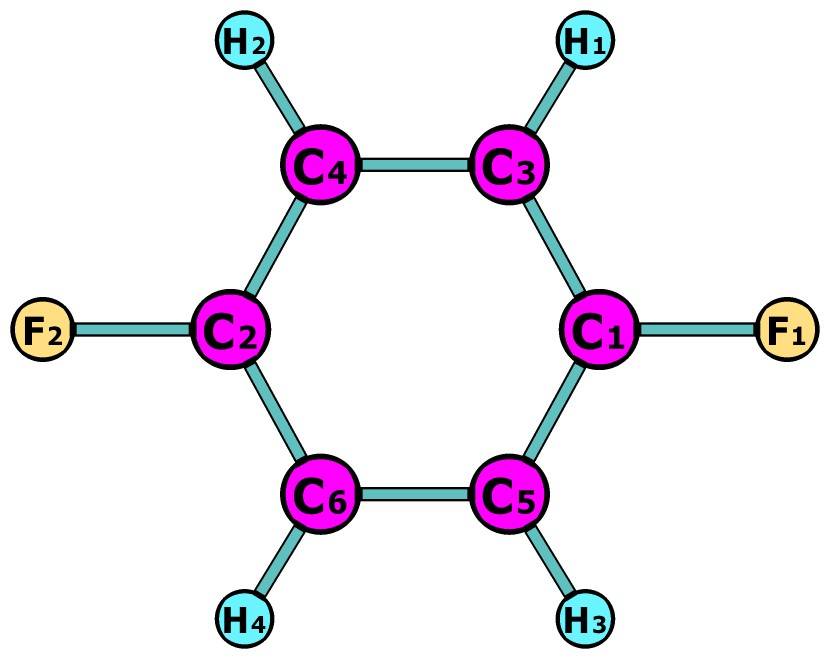
\includegraphics[scale=0.4]{fig/0.jpg}
\caption{Молекула 1,4-дифторбензола}
\end{figure}